\documentclass[a4paper, 12pt]{article}
\usepackage[utf8]{inputenc}
\usepackage[T2A]{fontenc}
\usepackage[english,russian]{babel}

\usepackage{authblk}  % для более гибкой работы с авторами
\usepackage{geometry} % если понадобится настроить поля
\usepackage{amssymb} % mathbb etc.
\usepackage{amsmath} % boldsymbol etc.
\usepackage{graphicx} % path to plot
\usepackage{algorithmic}
\usepackage{algorithm}
\usepackage{subcaption} % for subfigures
\usepackage[style=numeric-comp,sorting=none,maxnames=1,giveninits=true,doi=false,url=false,eprint=false]{biblatex} % for nice cites
\usepackage{cleveref}
\usepackage{etoolbox}

\defbibheading{bibliography}{
  \section*{\centering\small References}

  \vspace{-0.8em} % optional: reduces space after the title
}
\renewcommand*{\bibfont}{\small} % smaller than \small (usually 9pt)

\addbibresource{../article/draft_lib.bib}  % with .bib extension

% Title compactness
%\usepackage{titling}
%\setlength{\droptitle}{-2em}

% Custom bibliography style
\DeclareFieldFormat{title}{#1}
\DeclareFieldFormat{journaltitle}{#1}
\DeclareFieldFormat{volume}{\textbf{#1}}
\DeclareFieldFormat{number}{(#1)}
\DeclareFieldFormat{pages}{#1}

\renewbibmacro*{journal+issuetitle}{%
  \usebibmacro{journal}%
  \setunit*{\addcomma\space}%
  \iffieldundef{volume}{}{
    \printfield{volume}%
    \setunit{\addcolon\space}%
    \printfield{number}%
    \setunit{\addcolon\space}%
    \printfield{pages}}%
  \newunit}

\renewbibmacro*{volume+number+eid}{%
  \printfield{volume}%
  \setunit{\addcolon\space}%
  \printfield{number}%
  \setunit{\addcolon\space}%
  \printfield{pages}}

% Compact bibliography spacing
\setlength\bibitemsep{0pt plus 0.3ex}
\setlength\biblabelsep{0.5em}
\setlength{\bibnamesep}{0pt}
\setlength{\bibinitsep}{0pt}

\geometry{margin=2.5cm} % стандартные поля


% remove and for authors
\renewcommand\Authfont{\small} % размер шрифта для авторов
\renewcommand\Affilfont{\small} % размер шрифта для аффилиаций
\renewcommand\Authsep{, } % разделитель между авторами
\renewcommand\Authands{, } % разделитель между последним и предпоследним автором
\renewcommand\Authand{, } % для совместимости

% Reduce title spacing
\makeatletter
\renewcommand\maketitle{\par
  \begingroup
    \renewcommand\thefootnote{\@fnsymbol\c@footnote}%
    \def\@makefnmark{\rlap{\@textsuperscript{\normalfont\@thefnmark}}}%
    \long\def\@makefntext##1{\parindent 1em\noindent
            \hb@xt@1.8em{%
                \hss\@textsuperscript{\normalfont\@thefnmark}}##1}%
    \if@twocolumn
      \ifnum \col@number=\@ne
        \@maketitle
      \else
        \twocolumn[\@maketitle]%
      \fi
    \else
      \newpage
      \global\@topnum\z@
      \@maketitle
    \fi
    \thispagestyle{empty}\@thanks
  \endgroup
  \setcounter{footnote}{0}%
  \global\let\thanks\relax
  \global\let\maketitle\relax
  \global\let\@maketitle\relax
  \global\let\@thanks\@empty
  \global\let\@author\@empty
  \global\let\@date\@empty
  \global\let\@title\@empty
  \global\let\title\relax
  \global\let\author\relax
  \global\let\date\relax
  \global\let\and\relax
}
\makeatother

\makeatletter % small title and authors
\renewcommand{\maketitle}{
  \begin{center}
    \fontsize{15}{12}\selectfont
    \textbf{\@title} \\
    \vspace{0.5em}
    \@author \\
    \vspace{0.5em}
    \@date
  \end{center}
  \vspace{-0.5em}
}
\makeatother

% Title and author info (must be before \begin{document})
\title{\textbf{Differentially private modification of SignSGD}}
\author[]{A.Yu.~Kravatskiy}
\author[]{A.A.~Pliusnin}
\author[]{S.A.~Chezhegov}
\author[]{A.N.~Beznosikov}
\affil[]{Moscow Institute of Physics and Technology}
\date{} % убираем дату
\renewcommand{\and}{\\} % for authors
\newcommand{\eps}{\varepsilon}
\newcommand{\renyi}{R\'enyi}

\graphicspath{ {fig/} {../figs/} }

\begin{document}

\selectlanguage{english}
\noindent\foreignlanguage{russian}{УДК 519.676, 519.688}\vspace{-0.5em}
\maketitle
With large models requiring more and more data for training, federated learning has become more indispensable than ever. To use potentially sensitive user data for training the model, one has to guarantee its privacy. The gold standard for data privacy is \emph{$(\eps, \delta)$-differential privacy} \cite{Dwork2014} of mechanism, which guarantees that probabilities $p_1$ and $p_2$ of any response of the mechanism on datasets $D_1$ and $D_2$ respectively that differ only in one entry satisfy the relations $\frac{p_1}{p_2} \leq e^{\eps} + \delta$ and $\frac{p_2}{p_1} \leq e^{\eps} + \delta$. In federated learning, the mechanism returns all the outputs from the user, i.e. all the gradient data that they send to the server. For neural networks, standard parameters are $\eps = 1$, $\delta = 10^{-5}$. 

Another constraint of federated learning is the high communication cost. To reduce it, one can send not the whole gradient, but only the sign of each coordinate, thereby reducing the cost by a factor of $32/2 = 16$. The standard algorithm that utilizes this technique is SignSGD \cite{Bernstein2018}. This algorithm, which employs \emph{majority voting} among the workers, not only is communication-efficient but also is robust to heavy-tailed noise and converges with high probability \cite{Kornilov2025}.

Initially, we aimed to provide theoretical convergence guarantees for DP-SignSGD, a differentially private modification of SignSGD \cite{Jin2020}, following the approach in \cite{Kornilov2025}. However, upon closer examination, we found that the algorithm is not truly differentially private. The authors have shown $(\eps, \delta)$-privacy of a single iteration of DP-SignSGD, which means only $(T\eps, T\delta)$-privacy over $T$ iterations. Furthermore, they did not establish any convergence guarantees for DP-SignSGD.

Consequently, we had to construct our own DP-SignSGD. Like in \cite{Jin2020}, we use \emph{Gaussian mechanism} that ensures differential privacy by adding $\mathcal{N}(0,\sigma^2\mathbb{I}^d)$ noise. However, to make the most out of composition of mechanisms (a single mechanism returning a noised sign of the gradient) and to enhance privacy, we utilize \emph{Bernoulli subsampling}. In this scheme, at each iteration of the algoirthm, each entry of the dataset is sampled with probability $q$ and the gradients are computed only for the subsampled data. The resulting mechanism satisfies $(\alpha, \eps_R)$-\renyi\ differential privacy \cite{mironov2019SGM}, which is readily converted to $(\eps, \delta)$-privacy. We use the tightest bound for $\eps_R$ from \cite{mironov2019SGM}, which has only a numerical form:

\begin{equation}\label{eq:renyi_eps_guarantee}
\eps_R = \frac{1}{\alpha - 1} \log\left(\sum_{k=0}^{\alpha} {\alpha \choose k}  (1-q)^{\alpha-k}q^{k} \exp\left(\frac{k^2 - k}{2\sigma^2}\right)\right)
\end{equation}

To ensure privacy, the previously defined $\eps_R(q, \alpha, \sigma)$ must satisfy the following condition:
\begin{equation}\label{eq:renyi_eps_requirement}
\eps_R \leq \eps/T - \frac{\log 1/\delta}{T(\alpha - 1)}
\end{equation}

With $q$ being fixed, we use a grid search to find the minimal $\sigma$, as shown in \cref{fig:grid_sigma}.

\begin{figure}[h]
    \centering
    \begin{subfigure}[b]{0.39\textwidth}
        \centering
        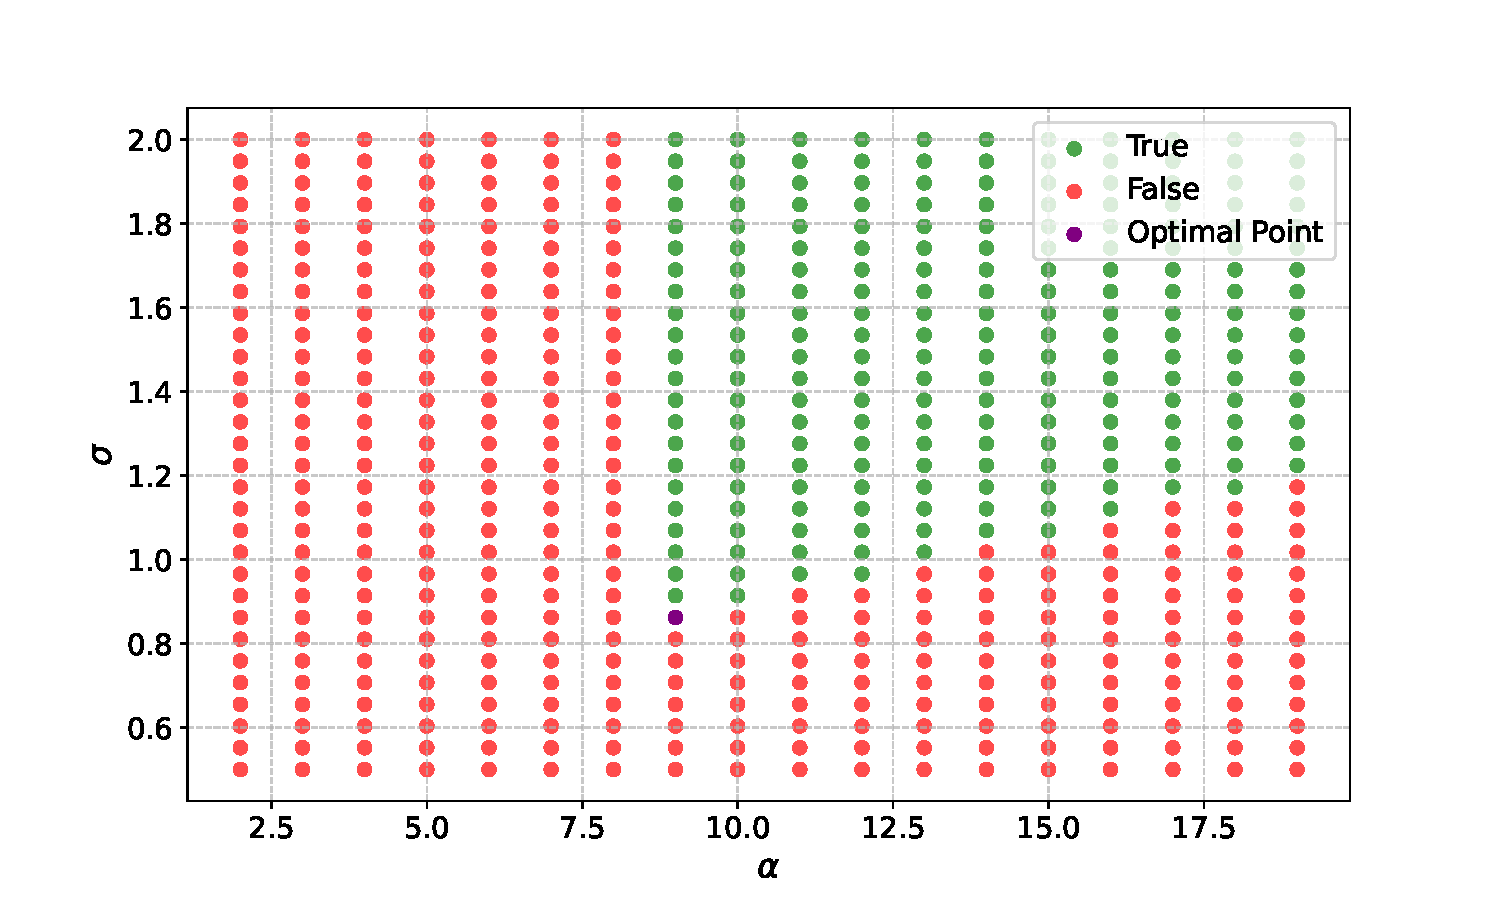
\includegraphics[width=\textwidth]{grid_sigma_to_pres.pdf}
        \caption{Finding the minimal $\sigma$, sampling rate $q = 1/300$, and $T = 1000$}
        \label{fig:grid_sigma}
    \end{subfigure}
    \hfill
    \begin{subfigure}[b]{0.6\textwidth}
        \centering
        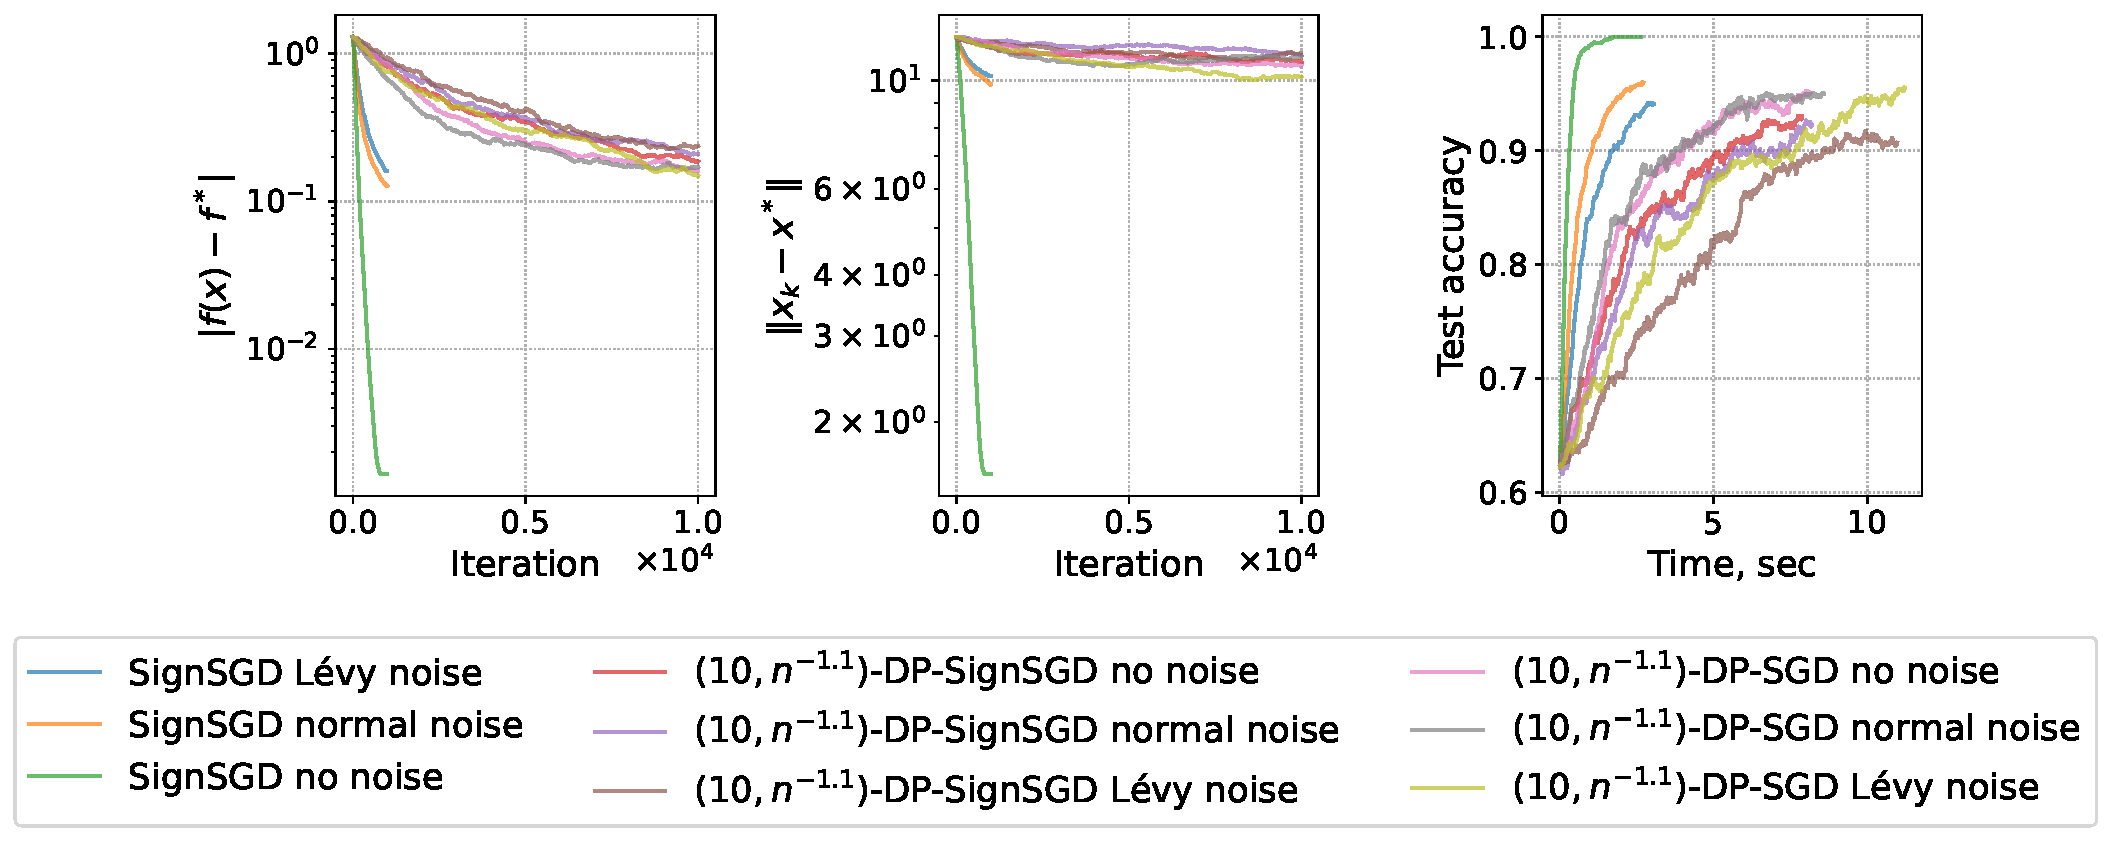
\includegraphics[width=\textwidth]{v28_constant_step/short/v28_constant_step_short.pdf}
        \caption{Logistic regression on UCI Mushroom Dataset with SGD, SignSGD, {\scriptsize DP-SIGN}SGD and different types of noise}
        \label{fig:logreg}
    \end{subfigure}
    \caption{Experimental results}
\end{figure}

Thus, we propose a new DP-SIGN compressor (see \cref{dp-sign-precise}) that defines a truly private variant of DP-SignSGD. We have tested it on a regularized logistic regression problem for binary classification. The results are presented in \cref{fig:logreg}.


\newcommand{\gradg}{\boldsymbol{g}}
\begin{algorithm}
    \caption{DP-SIGN compressor}
    \label{dp-sign-precise}
    \begin{algorithmic}
        \STATE \textbf{Input}: coordinate $w$, loss function $l$, user database $D$, $(\eps, \delta)$-privacy requirement, number of iterations $T$, sampling rate $q$.
        \STATE Prepare subsample $S$: add each element $(x, y) \in D$ with probability $q$.
        \STATE Compute the gradient $\gradg$ of the subsample for $\frac{1}{|S|}\sum_{(x,y)\in S}l(w;(x,y))$. If $S$ is empty, let $\gradg = 0$.
        % \STATE If $||\gradg||_2 > C$: $\gradg = C\frac{\gradg}{||\gradg||_2}$.
        \STATE Grid search $\sigma(q, T, \eps, \delta)$ to satisfy \eqref{eq:renyi_eps_guarantee} and \eqref{eq:renyi_eps_requirement}.
        \STATE $sign_{noised} = sign(\gradg) + \mathcal{N}(0,(2\sqrt{d}\sigma)^2\mathbb{I}^d)$
        % \STATE $\gradg_{priv}$ = $\gradg + \mathcal{N}(0,(C\sigma)^2\mathbb{I}^d)$
        \STATE \textbf{Output}: $sign(sign_{noised})$
    \end{algorithmic}
\end{algorithm}

We have also tested the algorithm on an MLP and a CNN for classifying handwritten digits from the MNIST dataset. On a single worker, we have achieved 70\% accuracy after 30,000 iterations with large $\sigma$, and 40\% accuracy after 2,000 iterations with small $\sigma$. The main obstacle to higher accuracy is the Gaussian noise inherent in private algorithms. Even with careful privacy accounting, it introduces a tradeoff between precision of a single iteration and the maximum number of iterations that still preserve privacy.

That being said, DP-SignSGD is likely more private than earlier stated bounds suggest. The sign mechanism, for instance, does not return all values in the range $[-1,1]$, but only 1 and -1, which inherently provides additional privacy guarantees. Furthermore, even the gradients may be partially private with respect to the user dataset. Estimating the impact of these aspects of the mechanism could lead to more feasible algorithms.

It is noteworthy that DP-SignSGD can be easily adapted to any tighter privacy guarantee: lower $\sigma$ or higher $T$ directly improves training. At present, the primary challenge concerning DP-SignSGD with Gaussian noise and Bernoulli subsampling is establishing theoretical guarantees of its convergence. To the best of our knowledge, none of the existing works provide a theoretical analysis of the application of the subsampling mechanism to optimization algorithms.

\vspace{-1.6em}
\printbibliography[heading=bibliography]


\end{document}
